\documentclass[12pt]{article}
\usepackage{preamble}

\pagestyle{fancy}
\fancyhead[LO,LE]{Теория вероятности}
\fancyhead[CO,CE]{29.10.2024}
\fancyhead[RO,RE]{Лекции Блаженова А. В.}

\fancyfoot[L]{\scriptsize исходники найдутся тут: \\ \url{https://github.com/pelmesh619/itmo_conspects} \Cat}

\begin{document}
    \subsection{Стандартное абсолютно непрерывное распределение}

    \subsubsection{I. Равномерное распределение}

    \Defs Случайная величина $\xi$ имеет равномерное распределение $\xi \in u(a, b)$, если ее плотность
    на этом отрезке постоянна

    Получаем функцию плотности $f_\xi(x) = \begin{cases}0, \quad x < a \\ \frac{1}{b - a}, \quad a \leq x < b \\ 0 \quad x \geq b\end{cases}$ \hfill {\scriptsize $\frac{1}{b - a}$ из усл. нормировки}

    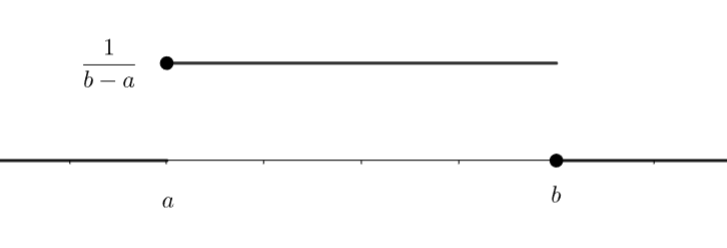
\includegraphics[height=4cm]{probtheory/images/probtheory_2024_10_29_1}

    Из этого функция распределения $F(x) = \int_{-\infty}^\infty f(x)dx = \begin{cases}0, \quad x < a \\ \frac{x - a}{b - a}, \quad a \leq x < b \\ 1 \quad x \geq b\end{cases}$

    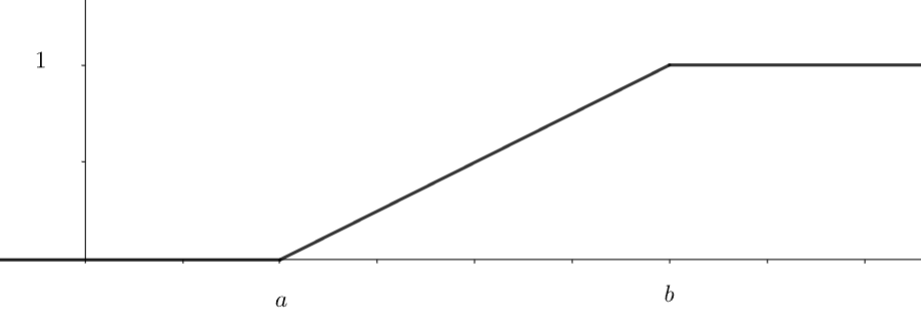
\includegraphics[height=4cm]{probtheory/images/probtheory_2024_10_29_2}

    \textbf{Числовые характеристики}:

    $E\xi = \int_{-\infty}^\infty x f(x) dx = \int_a^b x \frac{1}{b - a} dx = \frac{1}{b - a} \frac{x^2}{2} \Big|_a^b = \frac{b^2 - a^2}{2(b - a)} = \frac{a + b}{2}$

    $E\xi^2 = \int_{-\infty}^\infty x^2 f(x) dx = \int_a^b x^2 \frac{1}{b - a} dx = \frac{1}{b - a} \frac{x^3}{3} \Big|_a^b = \frac{b^3 - a^3}{3(b - a)} = \frac{b^2 + ab + a^2}{3}$

    $D\xi = E\xi^2 - (E\xi)^2 = \frac{b^2 + ab + a^2}{3} - \left(\frac{a + b}{2}\right)^2 = \frac{b^2 - 2ab + a^2}{12} = \frac{(b - a)^2}{12}$
    
    $\sigma = \sqrt{D\xi} = \frac{b - a}{2\sqrt{3}}$

    $p(\alpha < \xi < \beta) = \frac{\beta - \alpha}{b - a}$ при условии, что $\alpha, \beta \in [a, b]$

    \Nota Примеры равномерного распределения: задача со временем, датчики случайных чисел имеют стандартное равномерное распределение $u(0, 1)$

    \subsubsection{II. Показательное распределение}

    \Defs Случайная величина $\xi$ имеет показательное (или экспоненциальное) распределение с параметром $\alpha > 0$ (обозн. $\xi \in E_\alpha$),
    если ее плотность имеет вид:

    \[f_\xi(x) = \begin{cases}0, \quad x < 0 \\ \alpha e^{-\alpha x}, \quad x \geq 0\end{cases}\]

    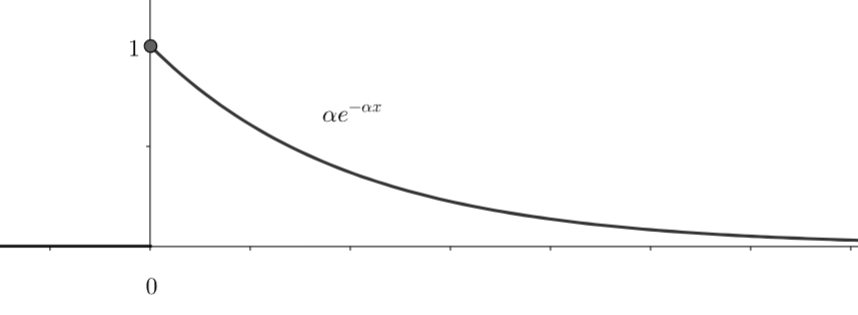
\includegraphics[height=4cm]{probtheory/images/probtheory_2024_10_29_3}

    Функция распределения $F_\xi(x) = \begin{cases}0, \quad x < 0 \\ \int_0^x \alpha e^{-\alpha x} = 1 - e^{-\alpha x}, \quad x \geq 0\end{cases}$

    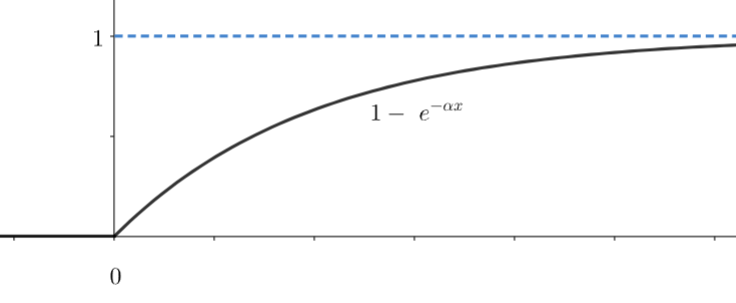
\includegraphics[height=4cm]{probtheory/images/probtheory_2024_10_29_4}

    \textbf{Числовые характеристики}:

    $E\xi = \int_{-\infty}^\infty x f(x) dx = \int_0^\infty x \alpha e^{-\alpha x} dx = \left[\begin{matrix}u = x & du = dx \\ dv = \alpha e^{-\alpha x} \alpha x & v = -e^{-\alpha x}\end{matrix}\right] = -xe^{-\alpha x} \Big|_0^\infty + \int_0^\infty e^{-\alpha x} dx = 
    -\lim_{x \to \infty} \frac{x}{e^{\alpha x}} - \frac{1}{\alpha} e^{-\alpha x} \Big|_0^\infty = -\lim_{x \to \infty} \frac{1}{\alpha e^{\alpha x}} - \frac{1}{\alpha} (\lim_{x \to \infty} e^{-\alpha x} - 1) = \frac{1}{\alpha}$


    $E\xi^2 = \int_{-\infty}^\infty x^2 f(x) dx = \int_0^\infty x^2 \alpha e^{-\alpha x} dx = \left[\begin{matrix}u = x^2 & du = 2xdx \\ dv = \alpha e^{-\alpha x} \alpha x & v = -e^{-\alpha x}\end{matrix}\right] = -x^2 e^{-\alpha x} \Big|_0^\infty + 2\int_0^\infty x e^{-\alpha x} dx = 
    \frac{2}{\alpha} \int_0^\infty \alpha x e^{-\alpha x} = \frac{2}{\alpha} E\xi = \frac{2}{\alpha^2}$

    $D\xi = E\xi^2 - (E\xi)^2 = \frac{2}{\alpha^2} - \left(\frac{1}{\alpha}\right)^2 = \frac{1}{\alpha^2}$
    
    $\sigma = \sqrt{D\xi} = \frac{1}{\alpha}$

    $p(\alpha < \xi < \beta) = F(b) - F(a) = e^{-a\alpha} - e^{-b\alpha} \quad\quad\quad a, b \geq 0$

    \Nota Из непрерывных случайных величин только показательная обладает свойством нестарения

    \begin{MyTheorem}
        \Ths $\letsymbol \xi \in E_\alpha$. Тогда $p(\xi < x + y \ | \ \xi > x) = p(\xi > y) \quad\quad \forall x, y > 0$
    \end{MyTheorem}

    \begin{MyProof}
        $\Box$

        $p(\xi < x + y \ | \ \xi > x) = p(\xi > y) = \frac{p(\xi > x + y, \xi > x)}{p(\xi > x)} = \frac{1 - p(\xi < x + y)}{1 - p(\xi < x)} = 
        \frac{1 - F(x + y)}{1 - F(x)} = \frac{e^{-\alpha(x + y)}}{e^{-\alpha x}} = e^{-\alpha y} = 1 - (1 - e^{-\alpha y}) = 1 - p(\xi < y) = p(\xi > y)$

        $\Box$
    \end{MyProof}

    \ExNs{1} Время работы надежной микросхемы до поломки

    \ExNs{2} Время между появлениями двух редких событий (через схему Пуассона)

    \Notas Применется в системах массового обслуживания, теория надежности


    \subsubsection{III. Нормальное распределение (Гауссовское)}

    \Def Случайная величина $\xi$ имеет нормальное распределение с параметрами $a$ и $\sigma^2$ (обозн. $\xi \in N(a, \sigma^2)$), если
    ее плотность имеет вид:

    \[f(x) = \frac{1}{\sigma \sqrt{2\pi}} e^{-\frac{(x - a)^2}{2\sigma^2}}, \quad -\infty < x < \infty\]

    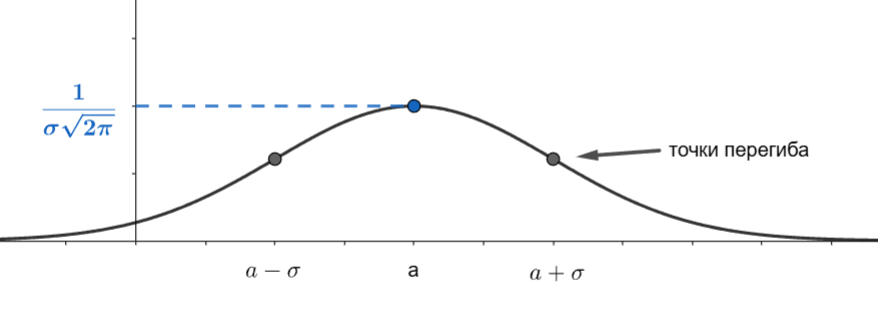
\includegraphics[height=4cm]{probtheory/images/probtheory_2024_10_29_5}

    Смысл параметров распределения: $a = E\xi$ - матожидание и медиана, $\sigma$ - СКО, а $D\xi = \sigma^2$

    Функция распределения: $F(x) = \frac{1}{\sigma \sqrt{2\pi}} \int_{-\infty}^x e^{-\frac{(t - a)^2}{2\sigma^2}} dt$

    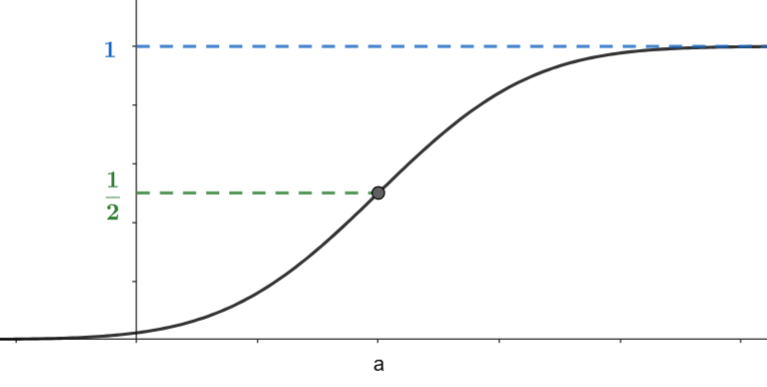
\includegraphics[height=4cm]{probtheory/images/probtheory_2024_10_29_6}

    Проверим корректность определения - условие нормировки. Покажем, что $\int_{-\infty}^\infty f(x)dx = 1$

    $\int_{-\infty}^\infty \frac{1}{\sigma \sqrt{2\pi}} e^{-\frac{(x - a)^2}{2\sigma^2}} dx = \left[\begin{matrix}t = \frac{x - a}{\sigma \sqrt{2}} & dt = \frac{dx}{\sigma\sqrt{2}} \\ t (\pm \infty) = \pm \infty & dx = \sigma\sqrt{2}dt\end{matrix}\right] = 
    \int_{-\infty}^\infty \frac{1}{\sigma\sqrt{2\pi}} e^{-t^2} \sigma\sqrt{2} dt = \frac{1}{\sqrt{\pi}} \int_{-\infty}^{\infty} e^{-t^2} dt = \frac{1}{\sqrt{\pi}} \sqrt{\pi} = 1$ - верно

    Ясно, что $m_k = \int_{-\infty}^\infty x^k f(x) dx = \int_{-\infty}^\infty x^k \frac{1}{\sigma \sqrt{2\pi}} e^{-\frac{(x - a)^2}{2\sigma^2}} dx$ - интеграл сходится абсолютно для любого $k$ (степень $e$ задавит полином)

    $E\xi = m_1 = \int_{-\infty}^\infty x^k \frac{1}{\sigma \sqrt{2\pi}} e^{-\frac{(x - a)^2}{2\sigma^2}} dx = a$ в силу симметрии

    Найдем дисперсию при помощи дифференцирования интеграла по параметру: 
    
    Из условия нормировки $\int_{-\infty}^\infty \frac{1}{\sigma \sqrt{2\pi}} e^{-\frac{(x - a)^2}{2\sigma^2}} dx = 1$

    $\frac{1}{\sqrt{2\pi}} \int_{-\infty}^\infty e^{-\frac{(x - a)^2}{2\sigma^2}} dx = \sigma$
    
    $\frac{1}{\sqrt{2\pi}} \int_{\infty}^\infty e^{-\frac{(x - a)^2}{2\sigma^2}} \left(-\frac{(x - a)^2}{2} (-\sigma^{-3})\right) dx = 1$
    
    $\frac{1}{\sigma\sqrt{2\pi}} \int_{\infty}^\infty (x - a)^2 e^{-\frac{(x - a)^2}{2\sigma^2}} dx = \sigma^2 = D\xi$, получаем, что $\sigma$ - СКО

    \mediumvspace

    \textbf{Стандартное нормальное распределение}

    \Def Стандартным нормальным распределением называется нормальное распределение с параметрами $a = 0, \sigma^2 = 1$: $\xi \in N(0, 1)$

    Плотность: $\phi(x) = \frac{1}{\sqrt{2\pi}} e^{-\frac{x^2}{2}}$ - функция Гаусса

    $E\xi = 0; \ D\xi = 1$

    Распределение: $F_0(x) = \frac{1}{\sqrt{2\pi}} \int_{-\infty}^x e^{-\frac{z^2}{2}} dz$ - функция стандартного нормального распределения

    Заметим, что $F_0(x) = \frac{1}{\sqrt{2\pi}} \int_{-\infty}^0 e^{-\frac{z^2}{2}} dz + \frac{1}{\sqrt{2\pi}} \int_0^x e^{-\frac{z^2}{2}} dz = \frac{1}{2} + \Phi(x)$, где $\Phi(x)$ - функция Лапласа

    Функция Лапласа нечетная и из соображения симметрии легко вычисляется для отрицательных $x$, однако большинство ПО используют $F_0(x)$
    
    \subsubsection{Связь между нормальным и стандартным нормальным распределениями}

    1) $\letsymbol \xi \in N(a, \sigma^2)$. Тогда $F_\xi(x) = F_0\left(\frac{x - a}{\sigma}\right)$

    \begin{MyProof}
        $\Box$
        
        $F_\xi(x) = \frac{1}{\sigma\sqrt{2\pi}} \int_{-\infty}^x e^{-\frac{(t - a)^2}{2\sigma^2}} dt = \left[\begin{matrix}z = \frac{t - a}{\sigma} & t = \sigma z + a & dt = \sigma dz \\ z (-\infty) = -\infty & z(x) = \frac{x - a}{\sigma} & \end{matrix}\right] = 
        \frac{1}{\sigma\sqrt{2\pi}} \int_{-\infty}^\frac{x - a}{\sigma} e^{-\frac{z^2}{2}} \sigma dz = \frac{1}{\sqrt{2\pi}} \int_{-\infty}^\frac{x - a}{\sigma} e^{-\frac{z^2}{2}} dz = F_0\left(\frac{x - a}{\sigma}\right)$
        
        $\Box$
    \end{MyProof}

    2) Если $\xi \in N(a, \sigma^2)$, то $\eta = \frac{\xi - a}{\sigma} \in N(0, 1)$ (процесс $\xi \to \eta$ называется стандартизацией)

    \begin{MyProof}
        $\Box$
        
        $F_\eta(x) = p(\eta < x) = p\left(\frac{\xi - a}{\sigma} < x\right) = p(\xi < \sigma x + a) = F_\xi(\sigma x + a) = F_0\left(\frac{\sigma x + a - a}{\sigma}\right) = F_0(x)$, так как $F_\eta(x) = F_0(x)$, то $\eta \in N(0, 1)$
        
        $\Box$
    \end{MyProof}

    3) $\letsymbol \xi \in N(a, \sigma^2)$. Тогда $p(\alpha < \xi < \beta) = \Phi\left(\frac{\beta - a}{\sigma}\right) - \Phi\left(\frac{\alpha - a}{\sigma}\right)$

    \begin{MyProof}
        $p(\alpha < \xi < \beta) = F_\xi(\beta) - F_\xi(\alpha) = F_0\left(\frac{\beta - a}{\sigma}\right) - F_0\left(\frac{\alpha - a}{\sigma}\right) = \Phi\left(\frac{\beta - a}{\sigma}\right) - \Phi\left(\frac{\alpha - a}{\sigma}\right)$
    \end{MyProof}

    4) Вероятность попадания в симметричный интервал (вероятность отклонения случайной величины от матожидания) 
    $p(|\xi - a| < t) = 2\Phi\left(\frac{t}{\sigma}\right)$

    \begin{MyProof}
        $p(|\xi - a| < t) = p(-t < \xi - a < t) = p(a - t < \xi < a + t) = \Phi\left(\frac{a + t - a}{\sigma}\right) - \Phi\left(\frac{a - t - a}{\sigma}\right) = \Phi\left(\frac{t}{\sigma}\right) - \Phi\left(-\frac{t}{\sigma}\right) = 2\Phi\left(\frac{t}{\sigma}\right)$
    \end{MyProof}

    \Notas Если через $F_0(x)$, то $p(|\xi - a| < t) = 2\F_0\left(\frac{t}{\sigma}\right) - 1$

    5) Правило 3 \enquote{сигм}: $p(|\xi - a| < 3\sigma) \approx 0.9973$ - попадание случайной величины нормального распределения в интервал $(a - 3\sigma, a + 3\sigma)$ близко к 1

    \begin{MyProof}
        $p(|\xi - a| < 3\sigma) = 2\Phi\left(\frac{3\sigma}{\sigma}\right) = 2\Phi(3) = 2 \cdot 0.49685 = 0.9973$
    \end{MyProof}

    6) Свойство линейности: если случайная величина $\xi \in N(a, \sigma^2)$, то $\eta = \gamma \xi + b \in N(a \gamma + b, \gamma^2 \sigma^2)$ (можем доказать при помощи свойств ранее, но мы докажем позже, используя другие методы)

    7) Устойчивость относительно суммирования: если случайные величины $\xi_1 \in N(a_1, \sigma_1^2), \xi_2 \in N(a_2, \sigma_2^2)$, и они независимы, то $\xi_1 + \xi_2 \in N(a_1 + a_2, \sigma^2_1 + \sigma^2_2)$

    \subsubsection{Коэффициенты асимметрии и эксцесса}

    \DefN{1} Асимметрией распределения называется число $A_s = E\left(\frac{\xi - a}{\sigma}\right)^3 = \frac{\mu^3}{\sigma^3}$

    \DefNs{2} Эксцессом распределения называется число $E_s = E\left(\frac{\xi - a}{\sigma}\right)^4 - 3 = \frac{\mu^4}{\sigma^4} - 3$

    \Notas Если случайная величина $\xi \in N(a, \sigma^2)$, то $A_s = E_s = 0$, таким образом, отличие этих характеристик от нуля характеризирует 
    степень отклонения распределения. Благодаря этим и другим параметрам, можно проверять на практике, является ли распределение нормальным 

\end{document}
